%-----------------------------------------------------------------------
% 
%-----------------------------------------------------------------------
%
%     
%
%
%%%%%%%%%%%%%%%%%%%%%%%%%%%%%%%%%%%%%%%%%%%%%%%%%%%%%%%%%%%%%%%%%%%%%%%%


\documentclass[twoside]{article}
\usepackage{amsmath,amsthm,amssymb,verbatim}

%     If your article includes graphics, uncomment this command.
\usepackage{graphicx}

%     If the article includes commutative diagrams, ...
%\usepackage[cmtip,all]{xy}

\usepackage{url}

\usepackage{fancyhdr}
\pagestyle{fancy}

\def\blfootnote{\xdef\@thefnmark{}\@footnotetext} 
\long\def\symbolfootnote[#1]#2{\begingroup%
\def\thefootnote{\fnsymbol{footnote}}\footnote[#1]{#2}\endgroup} 

	\addtolength{\oddsidemargin}{1cm}
	\addtolength{\evensidemargin}{-1cm}

\setcounter{page}{1}

\begin{document}

%     If you need symbols beyond the basic set, uncomment this command.
%\usepackage{amssymb}


\newtheorem{theorem}{Theorem}[section]
\newtheorem{lemma}[theorem]{Lemma}

\theoremstyle{definition}
\newtheorem{definition}[theorem]{Definition}
\newtheorem{example}[theorem]{Example}
\newtheorem{xca}[theorem]{Exercise}

\theoremstyle{remark}
\newtheorem{remark}[theorem]{Remark}

\numberwithin{equation}{section}


\date{}
\lhead[]{}
\chead[\underline{Deep Learning for Riemann Zeta}]{\it{O. Shanker}}
\rhead[]{}

% \title[short text for running head]{full title}
\title{\bf{Deep Learning for Riemann Zeta Function: Large Values and Karatsuba problem}}

\maketitle


%    author one information
% \author[short version for running head]{name for top of paper}
\author{{\textbf{O. Shanker}},}
\thanks{ Mountain View, CA 94041, U. S. A. email: oshanker@gmail.com}

\thispagestyle{fancy}

%    Abstract is required.
\begin{abstract}
Karatsuba, machine learning for 
the Riemann zeta function.
\end{abstract}
{\textbf {Keywords}:} Circular Unitary Ensemble, Riemann zeta, Value Distribution, Symmetry 
{\textbf {Mathematics Subject Classification (MSC)}:} 11M06, 11-04.


\symbolfootnote[0]{*}


\section{Introduction}

Karatsuba problem.  Many applications of machine learning in mathematics including Ref.~\cite{osneural}.


Ref.~\cite{Shanker 2018a,Shanker 2018b} studied 
the distribution of $Z(t)$ values 
at Gram points and showed  that  the  value

Ref.~\cite{Shanker 2020} showed that the value distribution of the Riemann zeta function 
can be expressed in terms of three  functions 
 which do not depend on the angle characterizing the Generalized Gram point. 

\section{\label{sec2}Materials and Methods}

\subsection{\label{seckaratsuba}Karatsuba Problem}
Karatsuba~\cite{K5} studied 

\begin{equation}
F(T; H)  \, = \, max_{|t-T| \le H} \zeta ( 0.5+it ) 
\label{eqRie}
\end{equation}


\subsection{\label{secwhy}Why Machine Learning?}

At large heights evaluating the Riemann zeta function  is a non-trivial task, requiring much computer time 
(and some knowledge of special techniques to find the roots).  It would be useful to apply
machine learning
as a guide to identify the T values where we can expect to see the behaviour of interest.
Ref~\cite{osneural} found that the behavior of the zeta function at Gram points 
is a good starting point to extract features for use in prediction. 
Ref.~\cite{Shanker 2018a} further showed that Gram points have interesting properties 
which distinguish them from random points on the critical line, supports the conclusion. 


It is known (Ref.~\cite{Shanker 2018b}) that the average value of the 

(Ref.~\cite{Shanker 2020}) that the probability distributions
Ref.~\cite{Shanker 2020} showed 
that the probability distributions 

\begin{figure*}
\centering
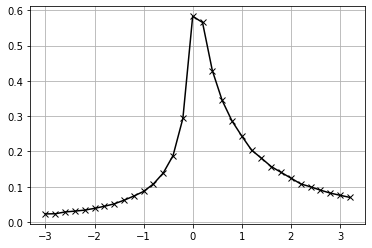
\includegraphics[width=0.8\textwidth]{1.png}
\caption[]{ 
  Distribution of $\zeta_{max}$. 
  }
\vspace{1mm}
\label{z1}
\end{figure*}

\begin{figure*}
\centering
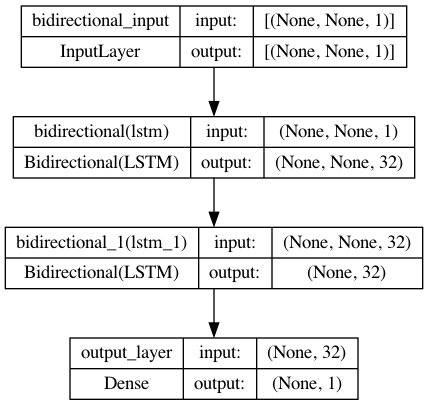
\includegraphics[width=0.8\textwidth]{2.png}
\caption[]{ 
  LSTM model. 
  }
\vspace{1mm}
\label{z2}
\end{figure*}

\begin{figure*}
\centering
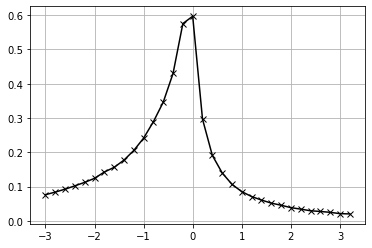
\includegraphics[width=0.8\textwidth]{3.png}
\caption[]{ 
  Training and Validation Mean Absolute Deviations.
  }
\vspace{1mm}
\label{z3}
\end{figure*}

\begin{figure*}
\centering
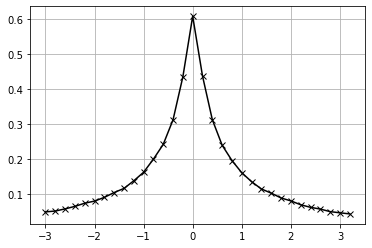
\includegraphics[width=0.8\textwidth]{4.png}
\caption[]{ 
  Comparision of model prediction with actual $\zeta_{max}$. 
  }
\vspace{1mm}
\label{z4}
\end{figure*}

\subsection{\label{seccalc}Calculating the sample values}

At large heights evaluating the Riemann zeta function  is a non-trivial task, requiring much computer time 

\section{\label{sec3}Results}

\subsection{\label{sec3.1} Choosing the Model}

Since the Riemann zeta studies were done at a
height $T = 10^{12}$, we use the well-known correspondence $N \thicksim \ln(T/2\pi)$ where $N$ 
is the size of the unitary matrix we should consider. Thus, we chose $N = 26$ for our
study.  We studied $500000$ gram intervals $U$ to generate the distributions.

have $N$ distinct CUE generalized Gram points spaced uniformly
around the unit circle.
The definition for the probability distribution is analogous to the Riemann zeta definition.

The CUE probability distributions satisfy (see Fig.~\ref{z1},~\ref{z2},~\ref{z3},~\ref{z4}) 

\begin{table}
\centering \(\begin{array}{cccccccccccc}

\hline
learning     &momentum  &epochs  \\
rate    &  &  \\
\hline
0.001 &0.895  & 15  \\
\hline
\end{array}\)
\caption{LSTM Model parameters (optimizer=tf.keras.optimizers.RMSprop)}
\label{tab:mean12}
\end{table}


\subsection{\label{relation}Training,  Model predictions}

For the Riemann zeta probability distributions, we found~\cite{Shanker 2020}
that the probability distributions at different $\phi$ can all be expressed in


\section{\label{conclusions}Conclusions}

We the Riemann zeta function.

\section*{Acknowledgments and Funding Statement}

 The study was done as an independent researcher. There was no
external funding.

\section*{Ethical Compliance}

 No procedures were performed  involving human participants in the study.

\section*{Data Availability Statement}

The computer programs used during the current study are
available from the corresponding author on reasonable request.

\section*{Conflict of Interest declaration} 

The authors declare that they have no affiliations with or involvement in any organization 
or entity with any financial interest in the subject matter or materials discussed 
in this manuscript.


\bibliographystyle{amsplain}
\begin{thebibliography}{10}

\bibitem{K5} A. A. Karatsuba, 
``Zero multiplicity and lower bound estimates of $|\zeta(s)|$",
{\it Funct.  Approx. Comment. Math.} {\bf35}(2006), 195–207

\bibitem{os6} O. Shanker, 
``Generalised Zeta Functions and Self-Similarity of Zero Distributions",
{\it J.  Phys. A} {\bf39}(2006), 13983-13997

\bibitem{osneural} O. Shanker, ``Neural Network prediction of Riemann zeta zeros''
{\it Advanced Modeling and Optimization}, {\bf 14}, 717-728, (2012). 

\bibitem{Shanker 2018a} O. Shanker, 
``Good to Bad Gram Point Ratio For Riemann Zeta Function",
{\it Experimental Mathematics} {\bf 30}, 76-85,
\url{tinyurl.com/mwd5uwc5}(2021)

\bibitem{Shanker 2018b} O. Shanker, 
``Symmetry properties of distribution of Riemann Zeta Function values on critical axis''
 report,
\url{tinyurl.com/47wj57b3}, 
(2018). 

\bibitem{Shanker 2020} O. Shanker, 
``Universality of Riemann Zeta Function value distribution on critical axis''
 report,
\url{tinyurl.com/yvbd2je6}, 
(2020). 




\end{thebibliography} 

\end{document}
